\documentclass[conference]{IEEEtran}
\IEEEoverridecommandlockouts
% The preceding line is only needed to identify funding in the first footnote. If that is unneeded, please comment it out.
\usepackage{cite}
\usepackage{amsmath,amssymb,amsfonts}
\usepackage{algorithmic}
\usepackage{graphicx}
\usepackage{textcomp}
\usepackage{xcolor}
\def\BibTeX{{\rm B\kern-.05em{\sc i\kern-.025em b}\kern-.08em
    T\kern-.1667em\lower.7ex\hbox{E}\kern-.125emX}}
\begin{document}

\title{Integration of FIWARE and IoT based Named Data Networking
    (IoT-NDN)
}

\author{\IEEEauthorblockN{Mohamed Ahmed Hail, Ian Pösse and Stefan Fischer }
    \IEEEauthorblockA{
        \textit{Institute of Telematics, University of Lübeck, Lübeck, Germany} \\
        \textit{\{hail, poesse, fischer\}@itm.uni-luebeck.de}
    }
}

\maketitle

\begin{abstract}
    The integration of IoT systems into various sectors like healthcare, smart cities, and energy is increasingly crucial, presenting challenges in mobility, energy use, and device memory.
    Early testing and evaluation of IoT systems are vital to reduce costs and efforts.
    FIWARE, an open-source IoT middleware, facilitates data transportation and big data tasks, playing a key role in this ecosystem.
    It offers a standardized architecture for managing context information in cloud-based IoT applications.
    This paper discusses the combination of FIWARE with IoT-NDN, a system based on the NDN protocol.
    IoT-NDN adapts NDN for IoT's specific needs. We present an approach to integrate FIWARE and IoT-NDN, enhancing IoT-NDN's implementation in existing applications.
    \newline
\end{abstract}

\begin{IEEEkeywords}
    Internet of Things (IoT); Named Data Networking (NDN); FIWARE Platform
\end{IEEEkeywords}

\section{Introduction}
The Internet of Things (IoT) is rapidly evolving, reshaping various sectors by providing advanced connectivity of devices, systems, and services. \cite[Alam, 2018]{b1}
This evolution brings significant benefits in areas such as healthcare, smart cities, and energy management, but also introduces complex challenges, particularly in terms of data management, system integration, and resource optimization.
At the heart of these challenges lies the need for efficient communication protocols and middleware solutions that can handle the vast and diverse nature of IoT data and devices.
FIWARE \cite[FIWARE Foundation]{b2}, an innovative, open-source IoT middleware, offers a comprehensive solution for managing context information in cloud-based IoT applications.
Its ability to handle big data tasks and provide a standardized architecture makes it a pivotal component in the IoT ecosystem.
However, to fully realize the potential of IoT, there is a need for seamless integration of such middleware solutions with efficient networking protocols.
IoT-based Named Data Networking (IoT-NDN), which is an adaptation of the Named Data Networking (NDN \cite[Zhang]{b7}) protocol, addresses these needs by focusing on data names rather than data locations.
This approach is particularly well-suited for IoT environments, where device mobility and varying network conditions are common. IoT-NDN simplifies data retrieval and dissemination processes, making them more efficient and reliable.
This paper delves into the integration of FIWARE with IoT-NDN, exploring how this combination can effectively address the challenges posed by IoT environments \cite[Sheng]{b6}.
We discuss the synergies between FIWARE's robust data handling capabilities and IoT-NDN's innovative approach to data networking. This integration not only enhances the efficiency of IoT systems but also opens up new possibilities for IoT applications across various sectors. By providing a detailed examination of this integration, we aim to contribute to the ongoing efforts in advancing IoT technologies and their applications.


\section{IoT-NDN and FIWARE}
IoT-NDN introduces a significant shift in internet protocol strategies by transitioning to a name-centered approach.
Instead of the conventional method, it utilizes systematically organized names for requesting data, which proves to be a more efficient methodology for Internet of Things (IoT) applications.
In parallel, the FIWARE platform offers a range of essential components specifically designed for IoT development.
These components include functionalities such as managing contextual information and seamlessly integrating big data services, thereby providing a robust and versatile framework for developing and enhancing IoT systems.

\section{Integration of FIWARE and IoT-NDN}
The integration of a FIWARE instance into IoT-NDN networks aims to facilitate bidirectional data access:
enabling FIWARE clients to retrieve information from IoT-NDN networks through FIWARE interfaces, and allowing NDN clients to access FIWARE context information via NDN requests.

\subsection{Architecture}
In order to align with FIWARE and its components, an adapter must partially implement the NGSIv2 API \cite[FIWARE developers]{b3}, optimally integrating a context provider with request forwarding capabilities.
This facilitates a bridge that translates between FIWARE and IoT-NDN requests.
At the thime of writing, this functionality is not fully realized in FIWARE Orion, the primary context provider \cite[FIWARE Orion]{b4}.
Consequently, data from IoT-NDN sensors is directed to FIWARE for storage and integration, supporting components dependent on data notifications, like Quantumleap for time-series database management.
Additionally, IoT-NDN devices require data access from the FIWARE context broker, necessitating the bridge to incorporate an IoT-NDN interface and establish a naming convention for mapping NDN requests to FIWARE entities.
The proposed FIWARE NDN adapter functions within both the IoT-NDN network and FIWARE ecosystem, requiring an NDN client and connectivity to the IoT-NDN router, with communication to FIWARE facilitated through the NGSIv2 API via HTTP requests.

\begin{figure}[htbp]
    \centerline{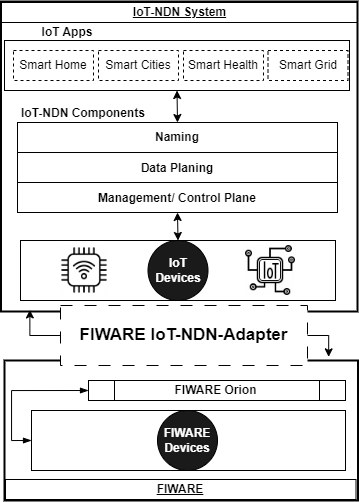
\includegraphics[scale=.4]{graph_draft.png}}
    \caption{ An Architecture of IoT-NDN and FIWARE Integration.}
    \label{iot-ndn-fiware}
\end{figure}

\subsection{Naming Convention}
In IoT-NDN networks, data addressing employs hierarchical names, reflecting tasks or scenarios, enabling targeted data requests. \cite[Hail, 2019]{b5}
FIWARE utilizes a similar structure with service-paths and entity IDs for entity identification.
The integration of IoT-NDN with FIWARE necessitates a mapping strategy where IoT-NDN device identifiers (comprising domain names, service-paths, and entity-IDs) correlate with FIWARE entities.
This system facilitates bi-directional information flow: IoT-NDN devices push data to a FIWARE adapter, updating corresponding entities, and also request data from FIWARE entities, irrespective of their presence in the IoT-NDN network.
Command-Infos in the naming structure provide additional context or command details.
\begin{figure}[tb]
    \centerline{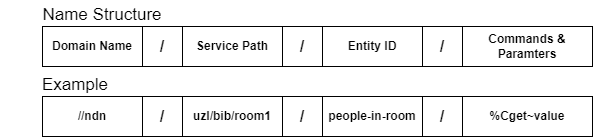
\includegraphics[scale=.4]{ndn-example.png}}
    \caption{An Example of Name-Structure of FIWARE and IoT-NDN.}
    \label{ndn-example}
\end{figure}
\vspace{6pt}
Let us consider an example: a device within the //ndn/ domain might be named ndn/uzl/bib/room1/amount-of-people, interfacing with a FIWARE adapter designated as uzl/bib/fiware.
This device could transmit data, such as the number of people in a room, at regular intervals (e.g., 1hz) to the FIWARE NDN adapter.
This is achieved by sending an interest packet like //ndn/uzl/bib/fiware/\%get~value,which the FIWARE adapter utilizes to update the corresponding data.
Similarly, when requesting data from a FIWARE entity, the request, prefixed with the adapter's name (//ndn/uzl/bib/fiware), reaches the adapter, which then retrieves and provides the requested data from the FIWARE domain.
This method allows for the emulation of non-existent sub-branches in the IoT-NDN structure, facilitating transparent interaction akin to standard NDN devices.
The command-info segment of the request can specify or filter requested attributes, such as the value in this instance.

\subsection{Interface Definition}
The proposed FIWARE NDN adapter functions as a relay, translating NDN messages to the FIWARE context broker's API.
This requires implementing two core methods: pushing data from IoT NDN devices to the context broker and requesting data from the broker within the IoT NDN network.
When data is pushed, the IoT NDN device's name is mapped to a corresponding FIWARE entity.
The data to be updated, encapsulated in the command-info block of the interest packet, is formatted into a JSON string.
The adapter then executes an HTTP PATCH request to the NGSIv2 API of the context broker, using specific routes to either update existing entities or create new ones if they don't exist, indicated by a 404 HTTP error code.
The service-path is decoded and included in the HTTP header to accurately identify the relevant entity.

\section{Conclusion}
This paper highlights the integration of FIWARE and IoT-based Named Data Networking (IoT-NDN), illustrating its potential in enhancing smart technologies.
We proposed a novel integration approach, centered on a mapping strategy and an IoT-NDN adapter, facilitating seamless integration into existing FIWARE applications.
This synergy enhances data monitoring in IoT-NDN networks and introduces advanced communication methods for various sectors.
Future work will focus on practical implementation, comprehensive evaluation, and optimization of this integrated system, especially for resource-limited IoT devices.

\begin{thebibliography}{00}
    \bibitem{b1} Alam, T. (2018). A reliable communication framework and its use in internet of things (iot). 3.
    \bibitem{b2} FIWARE Foundation, e.V. (2020c). The open source platform for our smart and digital future – fiware. Available at: https://www.fiware.org/.
    \bibitem{b3} Fiware developers - componentas. Fiware developers - componentas. Available at: https://www.fiware.org/developers/catalogue/.
    \bibitem{b4} FIWARE Orion Context Broker. FIWARE Orion Context Broker. Available at: https://fiware-orion.readthedocs.io/en/master/.
    \bibitem{b5} Hail, M. A. (2019). Iot-ndn: An IoT architecture via named data networking (ndn). In 2019 IEEE International Conference on Industry 4.0, Artificial Intelligence, and Communications Technology (IAICT), pages 74–80.
    \bibitem{b6} Sheng, Z., Yang, S., Yu, Y., Vasilakos, A. V., McCann, J. A., and Leung, K. K. (2013). A survey on the IETF protocol suite for the internet of things: standards, challenges, and opportunities. IEEE Wireless Communications, 20(6):91–98.
    \bibitem{b7} Zhang, L., Afanasyev, A., Burke, J., Jacobson, V., claffy, k., Crowley, P., Papadopoulos, C., Wang, L., and Zhang, B. (2014). Named data networking. SIGCOMM Comput. Commun. Rev., 44(3):66–73.
\end{thebibliography}
\end{document}
